\documentclass[12pt]{article}
\usepackage[english]{babel}
\usepackage{graphicx}
\usepackage[utf8]{inputenc}
\usepackage{blindtext} % Package to generate dummy text throughout this template 

\usepackage[sc]{mathpazo} % Use the Palatino font
\usepackage[T1]{fontenc} % Use 8-bit encoding that has 256 glyphs
\linespread{1.05} % Line spacing - Palatino needs more space between lines
\usepackage{microtype} % Slightly tweak font spacing for aesthetics

\usepackage{float} % picture position

\usepackage[english]{babel} % Language hyphenation and typographical rules

\usepackage[hmarginratio=1:1,top=32mm,columnsep=20pt]{geometry} % Document margins
\usepackage[hang, small,labelfont=bf,up,textfont=it,up]{caption} % Custom captions under/above floats in tables or figures
\usepackage{booktabs} % Horizontal rules in tables

\usepackage{lettrine} % The lettrine is the first enlarged letter at the beginning of the text

\usepackage{enumitem} % Customized lists
\setlist[itemize]{noitemsep} % Make itemize lists more compact

\usepackage{abstract} % Allows abstract customization
\renewcommand{\abstractnamefont}{\normalfont\bfseries} % Set the "Abstract" text to bold
\renewcommand{\abstracttextfont}{\normalfont\small\itshape} % Set the abstract itself to small italic text

\usepackage{titlesec} % Allows customization of titles
\renewcommand\thesection{\Roman{section}} % Roman numerals for the sections
\renewcommand\thesubsection{\roman{subsection}} % roman numerals for subsections
\titleformat{\section}[block]{\large\scshape\centering}{\thesection.}{1em}{} % Change the look of the section titles
\titleformat{\subsection}[block]{\large}{\thesubsection.}{1em}{} % Change the look of the section titles

\usepackage{fancyhdr} % Headers and footers
\pagestyle{fancy} % All pages have headers and footers
\fancyhead{} % Blank out the default header
\fancyfoot{} % Blank out the default footer
\fancyhead[C]{RVC Applied AI $\bullet$ 2022 $\bullet$ MIPT} % Custom header text
\fancyfoot[RO,LE]{\thepage} % Custom footer text

\usepackage{titling} % Customizing the title section

\usepackage{hyperref} % For hyperlinks in the PDF
\usepackage{amssymb,amsmath,amsthm}

\theoremstyle{plain}
\newtheorem{proposition}{Proposition}
\theoremstyle{definition}
\newtheorem{definition}{Definition}
\newtheorem{notation}{Notation}
\newtheorem{example}{Example}
\DeclareMathOperator{\sign}{sign}

\setlength{\droptitle}{-4\baselineskip} % Move the title up

% Keywords command
\providecommand{\keywords}[1]
{
  \small	
  \textbf{\textit{Keywords}} #1
}

\title{\textbf{\Huge{Machine learning approach to startup success prediction}}}
\author{%
\textsc{Pavlov D.} \\[1ex] 
\normalsize MIPT\\ 
\normalsize \href{mailto:dima-pavlov@phystech.edu}{dima-pavlov@phystech.edu}
\and 
\textsc{Moiseev A.} \\[1ex] 
\normalsize MIPT
\and 
\textsc{Ammosov Y.} \\[1ex] 
\normalsize MIPT
}


\date{\today}

\renewcommand{\maketitlehookd}{

\begin{abstract}
% - wide-range field of the investigated problem,
% - narrow problem to focus on,
% - features and conditions of the problem,
% - the novelty (please not exaggerate),
% - application to illustrate with (put the results here later).

This paper deals with a model for predicting the success of startups based on data about companies from CrunchBase and data about founders and investors associated with the company from LinkedIn. Unlike CrunchBase, where we have data with a clear structure, in a social network, data is filled in in the free form. In the last decade, natural language processing has shown good results when working with unstructured data. The approach for model construction using data about founders is new for the venture industry.
\noindent  \\

\keywords{Venture Capital · Natural Language Processing}

\end{abstract}

}

\begin{document}

\maketitle

\clearpage

\section{Introduction}

% - the research goal (and its motivations),
% - the object of research (introduce main termini),
% - the problem (what is the challenge),
% - methodology: literature review and state-of-the-art
% - the project tasks,
% - the proposed solution, its novelty and advantages,
% - the profs and cons of recent works,
% - goal of the experiment, set up, data sets, workflow.

%There is a lot of unstructured information on the Internet that is useful for people who are professionally-looking for new projects and ideas. Data mining in venture business allows to collect big data usefull for prediction models from social networks and news. 

The number of startups born every day is growing from year to year. 
The growth leads to an increase in the load on the pipeline of a venture capital company. 

\subsection{Link review}

\begin{enumerate}
    \item \href{https://www.mdpi.com/2071-1050/13/4/2242/htm}{Econometric Estimation of the Factors That Influence Startup Success}
\end{enumerate}

\section{Data}
    
\begin{itemize}
    \item Raw data from LinkedIn pages
    \item CrunchBase startups base
\end{itemize}

\section{Data Preparation}

\subsection{"Education field of study" field}

\begin{itemize}
    \item Handmade labels of "education field of study"
    \item Labeling using ML algorithms
   
\end{itemize}

\pagebreak

\section{Research tracks}

\subsection{Statistical hypotheses}

\begin{enumerate}
    \item The field of study associated person correlates with the success of a startup
    
    \begin{figure}[H]
      \centering
      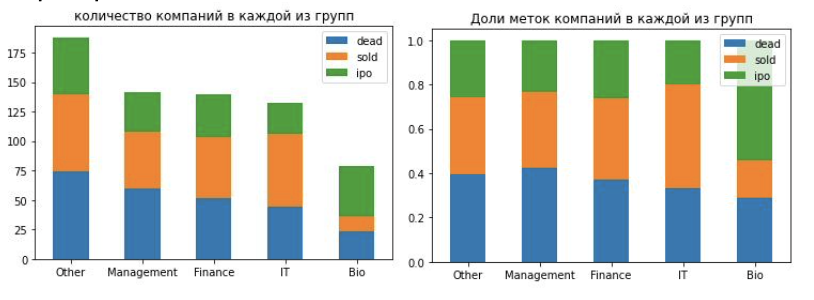
\includegraphics[width=120mm]{figures/collection/EFOFS-success.png}
      \label{fig:gd}
      \caption{Education of associated person and startup success}
    \end{figure}
    
    Biologists are statistically significantly more likely to IPO
    
    \item Top 10 characteristic skills of each of the areas of study. TF-iDF for skills in each of "education of study group".
    
    \begin{figure}[H]
      \centering
      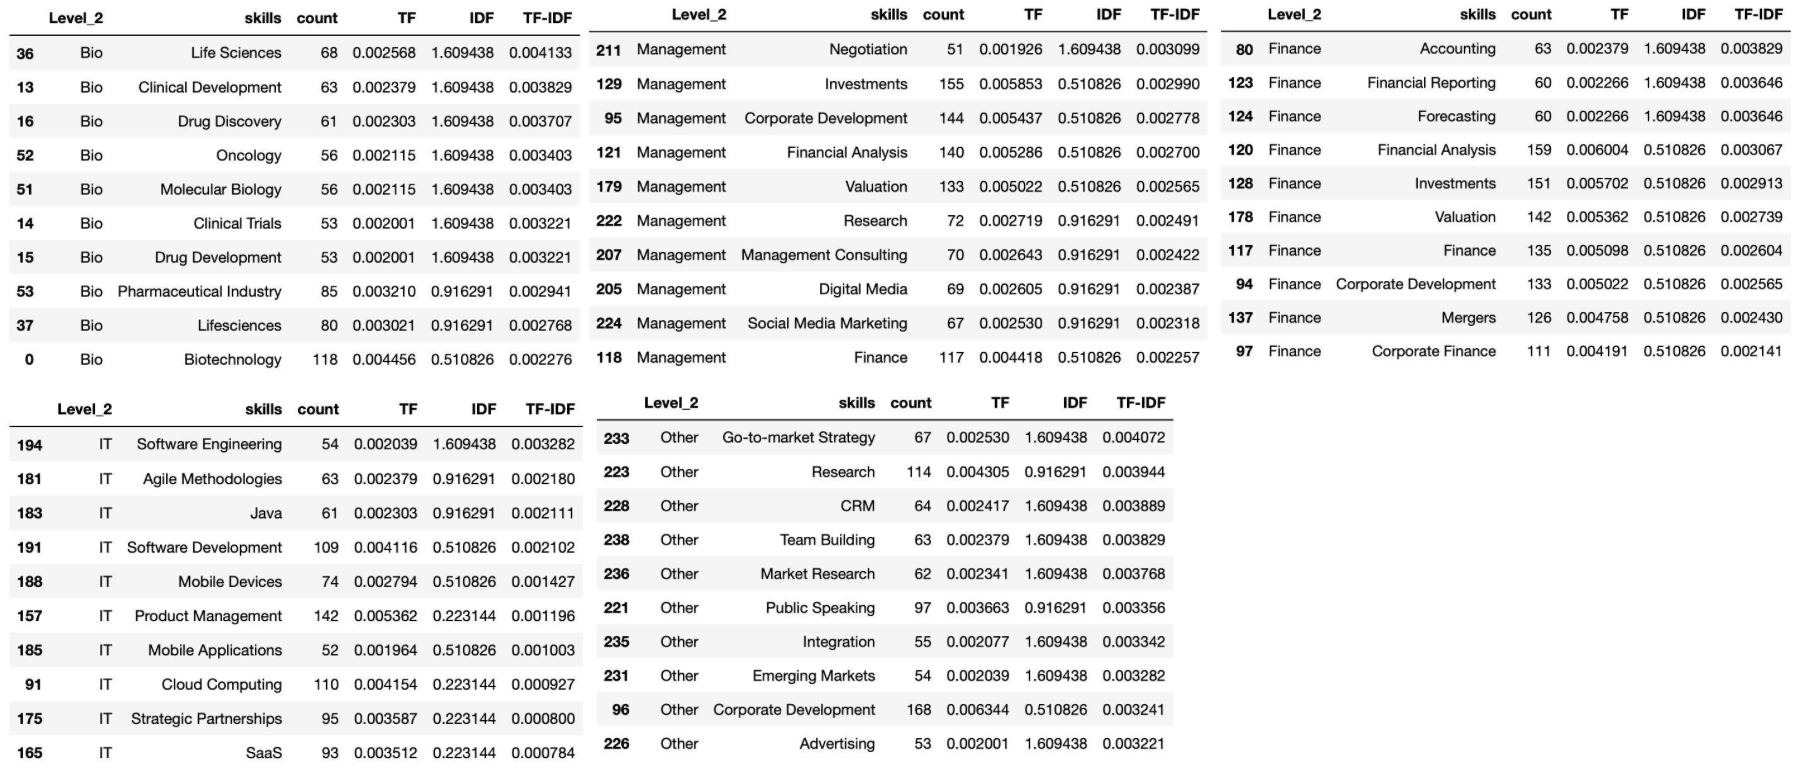
\includegraphics[width=160mm]{figures/collection/Characteristic-skills-per-group.png}
      \label{fig:gd}
      \caption{Characteristic skills for education field of study group}
    \end{figure}
    
    Just a fact for handmade labeling
    
    \item Statistics of "education field of study" groups by city.
    
    \begin{figure}[H]
      \centering
      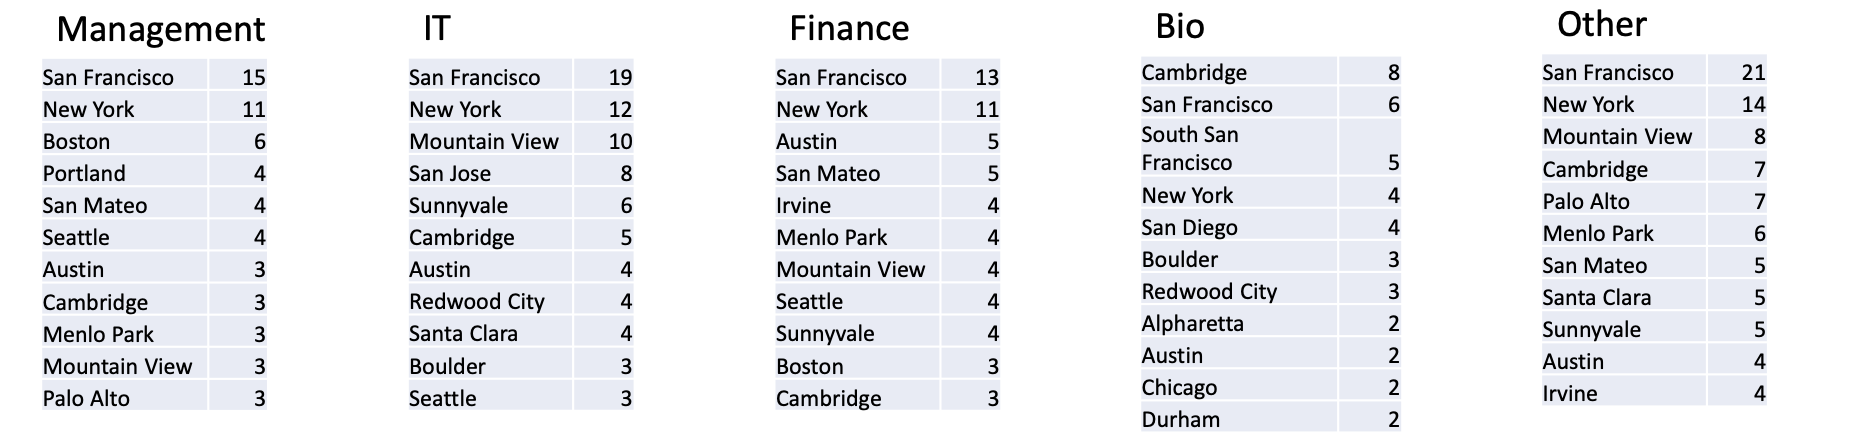
\includegraphics[width=140mm]{figures/collection/City-efofs-group.png}
      \label{fig:gd}
      \caption{Education field of study group distribution by city}
    \end{figure}
    
    Just a fact for handmade labeling
    
    \item The more diverse experiences person associated with a startup has, the more successful the startup is.
    
    \begin{figure}[H]
      \centering
      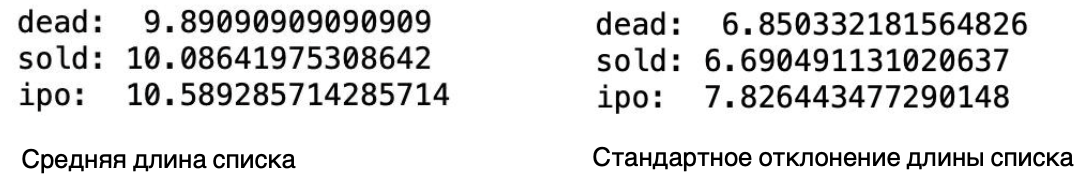
\includegraphics[width=120mm]{figures/collection/Different-experience-and-success.png}
      \label{fig:gd}
      \caption{Diverse experience and startup success}
    \end{figure}
    
    No statistically significantly results
    
    \item Correlation between the number of people leaving the company and the success of the startups associated with the people.
    
    \begin{figure}[H]
      \centering
      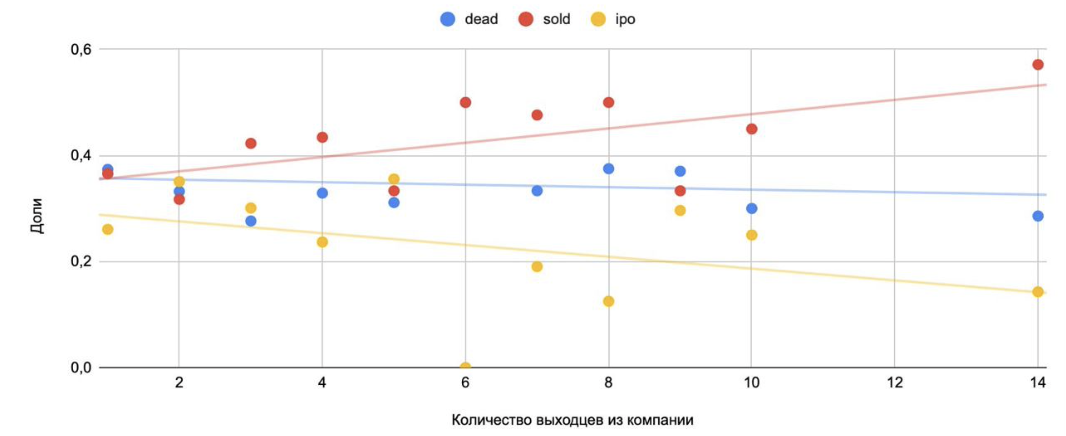
\includegraphics[width=120mm]{figures/collection/Count-of-exists-and-success.png}
      \label{fig:gd}
      \caption{The company size and startup success}
    \end{figure}
    
    No statistically significantly results, but there are some trends. Need to normalize the number of employees in the company
    
\end{enumerate}

\subsection{Data structuring}

\begin{enumerate}
    \item Handmade labels of "education field of study" strings in LinkedIn profile.
    
    \item NLP based methods for representation strings from LinkedIn profile as embeddings
    
    \begin{enumerate}
        \item Lemmatization and stemming to reduce strings to a common form
        
        Just bad resuls..
        
        \item 3-gram generation to count frequency between grams and classes from manual markup
        
        Just bad resuls..
        
        \item Embeddings generated by LaBSE (NN based on BERT) have Word2Vec property
        
        \begin{figure}[H]
          \centering
          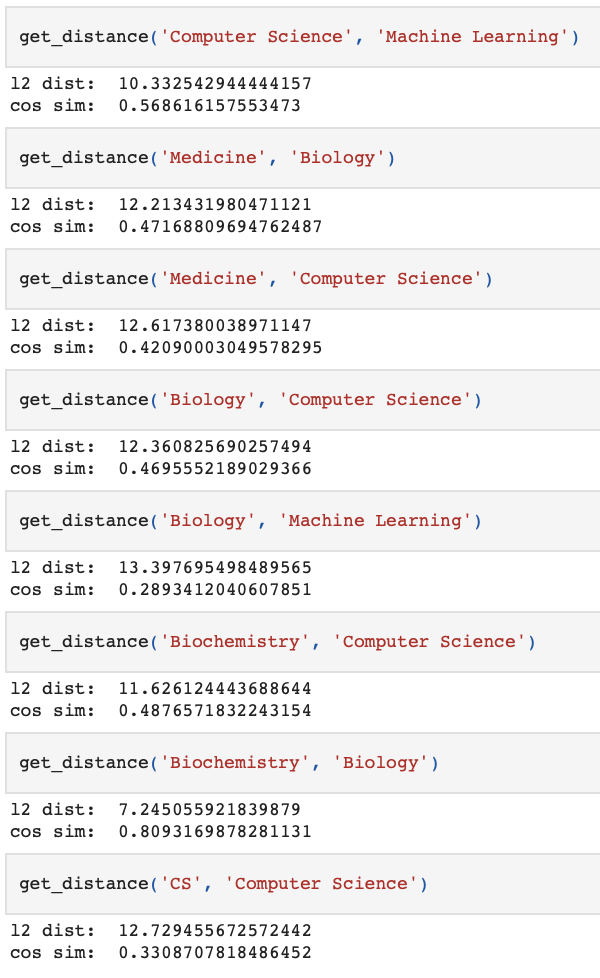
\includegraphics[width=70mm]{figures/collection/Word2Vec-LaBSE.png}
          \label{fig:gd}
          \caption{Word2Vec property of embeddings}
        \end{figure}
        
        The more L2 -- the further strings.
        
        The more cos simmilarity -- the closer strings.
        
        \item Clusterization of embeddings generated by LaBSE using kMeans
        
        \begin{figure}[H]
          \centering
          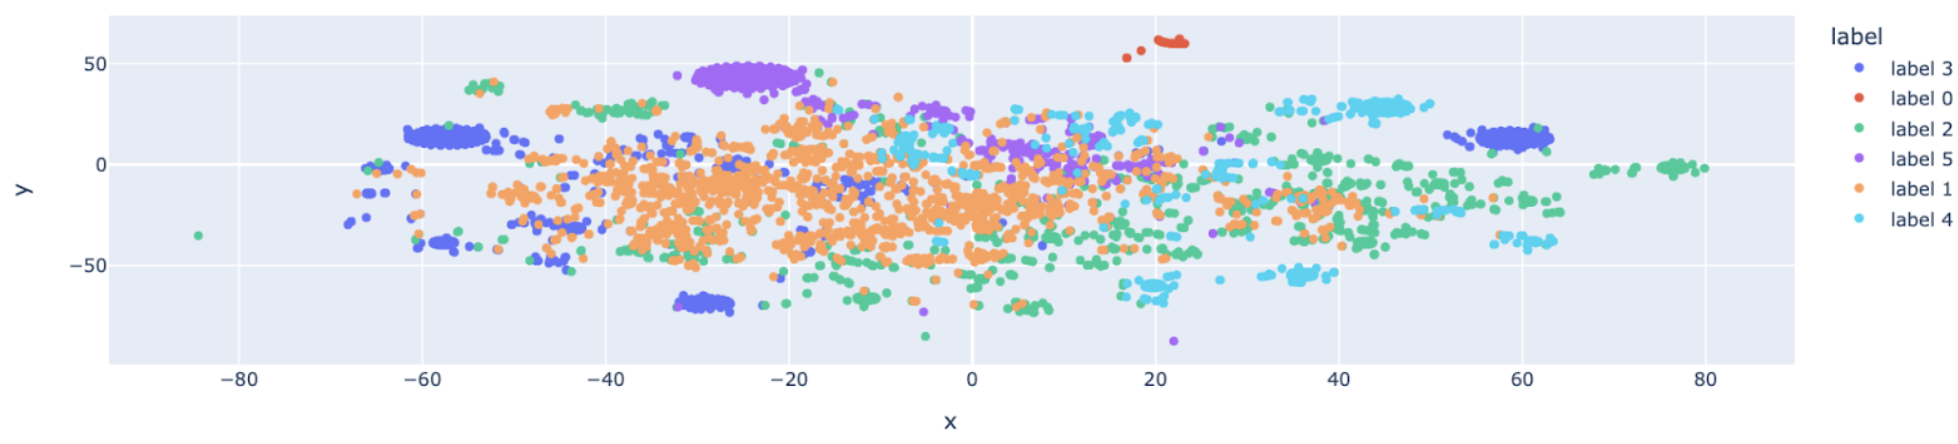
\includegraphics[width=140mm]{figures/collection/kMeans-LaBSE.png}
          \label{fig:gd}
          \caption{kMeans LaBSE and TSNE}
        \end{figure}
        
        \begin{figure}[H]
          \centering
          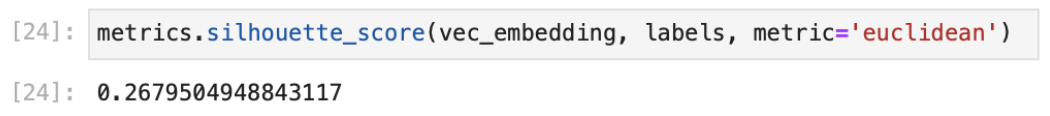
\includegraphics[width=100mm]{figures/collection/kMeans-LaBSE-metric.png}
          \label{fig:gd}
          \caption{The Silhouette Coefficient}
        \end{figure}
        
        Since the value is sufficiently greater than zero, the clusterer is more likely to separate classes than not
    
        \item Using generated embeddings by LaBSE, SVC predicts education field of study class from handmade labels
        
        \begin{figure}[H]
          \centering
          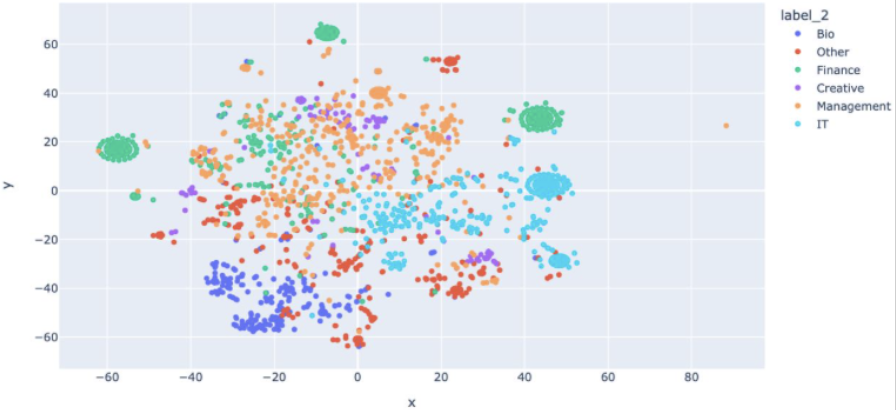
\includegraphics[width=140mm]{figures/collection/Embeddings-handmade.png}
          \label{fig:gd}
          \caption{TSNE embeddings}
        \end{figure}
        
        \begin{figure}[H]
          \centering
          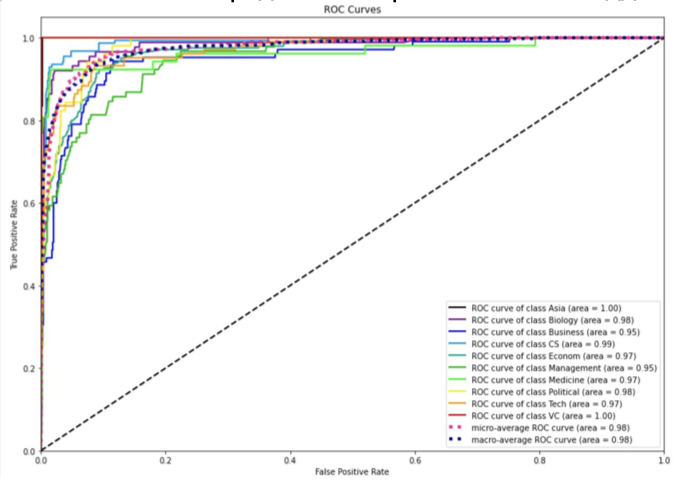
\includegraphics[width=120mm]{figures/collection/ROC-SVC.png}
          \label{fig:gd}
          \caption{ROC curve for SVC}
        \end{figure}
        
        Pretty good quality. However, the model may be unstable on new data.
        
    \end{enumerate} 
    
    \item NLP methods for sentence similarity task: strings from LinkedIn profile are ranked according to the metric of similarity to one of the classes: Manager, Computer Science, Finance, Biology, Other
    
    \begin{figure}[H]
      \centering
      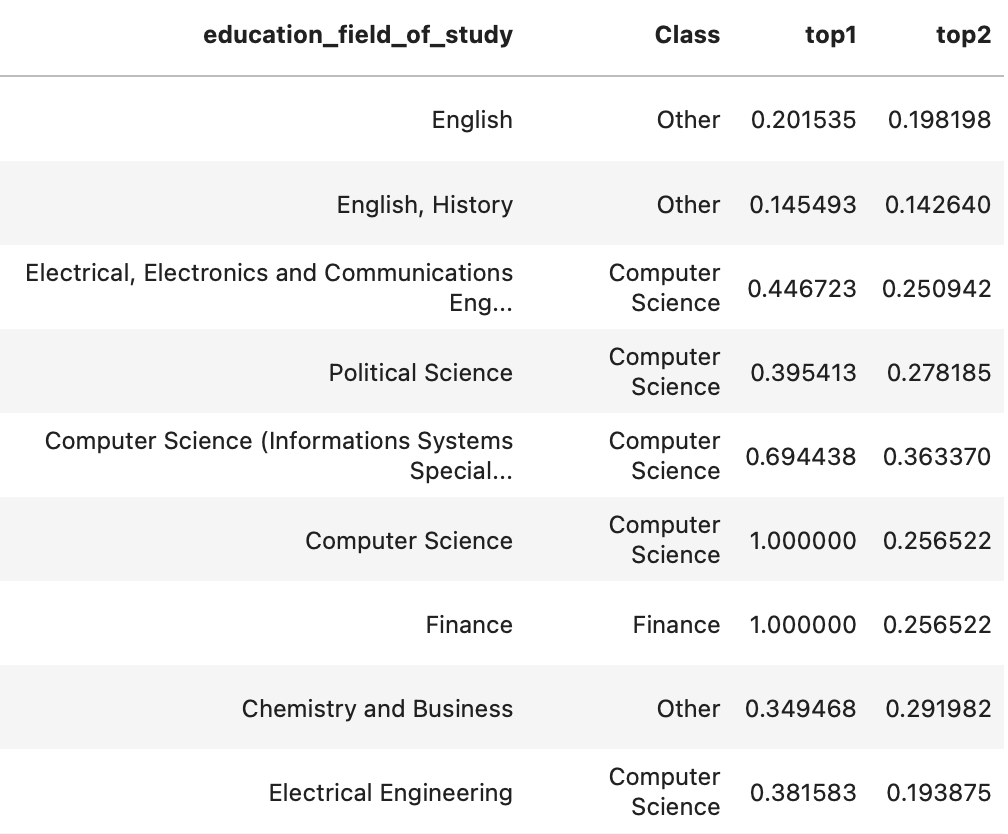
\includegraphics[width=100mm]{figures/collection/Similarity-rank.png}
      \label{fig:gd}
      \caption{Similarity between "education field of study" strings and one of strings: Computer Science, Management, Finance, Biology}
    \end{figure}
    
    For large datasets, this model may be sufficient. However, there are some serious mistakes: "Political Science" and "Computer Science". This happened because I chose the cutoff threshold so that "Electrical Engineering" sim "Computer Science".I think you need to use partitioning into more groups and increase the cutoff threshold.
    
\end{enumerate}

\end{document}